\section{Event Layout}
\label{app:params}
Table~\ref{tab:events} lists the simulated events for all six scenarios (positions
in world metres; $I_e$ is the base intensity). The patrol waypoints are
$(13,-8)$, $(13,10)$, $(0,11)$, $(-8,5)$, $(-10,-10)$. The remaining method and
simulation parameters are given in Table~\ref{tab:hyper}.

\begin{table}[h]
\centering
\caption{Simulated events for all six scenarios (positions in world metres;
$I_e$ is the base intensity). In \emph{dyn-hazard} the repulsive event is
co-located with the anomaly and \emph{activates}---starts being published to
both the reactive and keepout channels---only when the robot reaches
$\le3$\,m of its true position ($r_{\mathrm{act}}$), modelling a hazard that
emerges during an ongoing investigation.}
\label{tab:events}
\begin{tabular}{llccc}
\hline
\textbf{Scenario} & \textbf{Type} & $\bm{x}$ & $\bm{y}$ & $\bm{I_e}$\\
\hline
default & thermal (attr.)  & 10   & 10  & 0.85\\
        & thermal (attr.)  & 0    & 15  & 0.91\\
        & acoustic (attr.) & $-5$ & 5   & 0.72\\
        & hazard (rep.)    & 2    & $-13$ & 0.90\\
\hline
adverse & thermal (attr.)  & 10   & 10  & 0.85\\
        & acoustic (attr.) & 7    & 8   & 0.78\\
        & thermal (attr.)  & 0    & 15  & 0.91\\
        & acoustic (attr.) & $-5$ & 5   & 0.72\\
        & thermal (attr.)  & $-8$ & 8   & 0.80\\
        & hazard (rep.)    & 2    & $-13$ & 0.90\\
\hline
route- & thermal (attr.)  & 10   & 10  & 0.85\\
hazard  & thermal (attr.)  & 0    & 15  & 0.91\\
        & acoustic (attr.) & $-5$ & 5   & 0.72\\
        & hazard (rep.)    & $1.5$ & $-9$ & 0.90\\
\hline
conflict& thermal (attr.)  & 10   & 10  & 0.85\\
        & thermal (attr.)  & 0    & 15  & 0.91\\
        & acoustic (attr.) & $-5$ & 5   & 0.72\\
        & acoustic (attr.) & 2    & $-13$ & 0.95\\
        & hazard (rep.)    & 2    & $-13$ & 0.70\\
\hline
dyn-    & thermal (attr.)  & 2    & $-13$ & 0.90\\
hazard  & hazard (rep.)$^\dagger$ & 2 & $-13$ & 0.90\\
\hline
%% P7: o cenario conflict-marginal (CM) nao constava, embora a Secao V-F o use.
conflict- & thermal (attr.)  & 10   & 10  & 0.85\\
marginal  & thermal (attr.)  & 0    & 15  & 0.91\\
          & acoustic (attr.) & $-5$ & 5   & 0.72\\
          & acoustic (attr.) & 4    & $-10.5$ & 0.95\\
          & hazard (rep.)$^\ddagger$ & 0 & $-12$ & 0.52\\
\hline
\multicolumn{5}{l}{\footnotesize $^\dagger$ activates only within
  $r_{\mathrm{act}}=3$\,m of the true position.}\\
\multicolumn{5}{p{0.9\columnwidth}}{\footnotesize $^\ddagger$ calibrated so that the
hazard sits just above the eligibility threshold along the approach the planner
actually takes: at the measured approach distance of ${\approx}3.7$\,m,
Eq.~\eqref{eq:intensity} yields ${\approx}0.33$ against $\theta_{\mathcal{H}}=0.30$.
The base value $0.52$ keeps the hazard eligible throughout $d\in[3.5,4.0]$\,m, so the
scenario does not depend on an exact approach geometry. The anomaly at $(4,-10.5)$
is \emph{not} co-located with the hazard: it is the fourth, suppressible target.}\\
\end{tabular}
\end{table}

\section{Secondary Statistical Comparisons}
\label{app:stats}
Table~\ref{tab:stats} in Section~\ref{sec:results} reports the confirmatory family
of this submission---three contrasts $\times$ five outcomes, Holm-corrected within
those fifteen tests and shown in full. The comparisons that formed the
confirmatory family of the \emph{previous} submission are kept separately in
Table~\ref{tab:legacystats} and reported uncorrected, so that only one family
carries a multiplicity correction. Table~\ref{tab:allstats} below reports the remaining
comparisons of the study, which are of a different nature and are therefore kept
separate: \emph{equivalence} checks (the $\eta$ ablation, where a \emph{non}-effect
is the expected and desired outcome) and \emph{robustness/cost} checks
(perception noise and the adverse scenario). For the mission-time rows the equivalence evidence
is a formal two one-sided test (TOST) against a pre-declared $\pm5$~s margin,
\emph{not} the absence of a significant difference: the $\eta$-ablation rows
(E0~vs~E2/E3/E4) are equivalent ($p_{\mathrm{TOST}}<10^{-6}$). The TOST requires
positive variance and is therefore \emph{not applicable} to constant-count rows:
under moderate noise (E3~vs~N1) the two arms are all $3.0$, so we report
\emph{identical observed performance} rather than a statistical equivalence
(an absence of dispersion in two small ceiling-valued samples does not demonstrate
population equivalence); under high noise (E3~vs~N2) the counts differ
($\Delta=-0.67$, $p=0.009$), the signature of the graceful degradation of
Section~\ref{sec:robustness}. Difference tests are Mann--Whitney $U$ (two-sided): the exact $U$ distribution for
untied samples with $n_1+n_2\le20$, a two-sided exact permutation $p$ for fully
separated constant arms, the tie-corrected normal approximation when ties are
present, and $p{=}1.00$ when the two arms are identical; the $95\%$ CI is the
bootstrap interval of the mean difference $\Delta$ (second minus first
configuration).

%% P1 do parecer de 2026-10-16: a familia confirmatoria ANTERIOR (7 testes)
%% saiu da Tabela 4, que agora traz so a familia desta submissao. Fica aqui,
%% rotulada como historica e SEM correcao, para nao haver duas familias
%% confirmatorias simultaneas no artigo.
\begin{table}[t]
\centering
\caption{Comparisons that formed the confirmatory family of the \emph{previous}
submission, retained for continuity. They are \emph{not} part of this
submission's Holm family (Table~\ref{tab:stats}) and their $p$-values are
therefore reported uncorrected. E1 is the fixed patrol, RHB the fixed patrol on
the on-route hazard, and APF the potential-field baseline.}
\label{tab:legacystats}
\footnotesize
\setlength{\tabcolsep}{4pt}
\begin{tabular}{llccccc}
\hline
\textbf{Pair} & \textbf{Outcome} & $\bm{n}$ & $\bm{\Delta}$ & $\bm{\delta}$ &
\textbf{95\% CI} & $\bm{p}$\\
\hline
%% GERADO por tabela_confirmatoria_tex.py --legacy. Nao editar a mao.
E1 vs E3    & Anomalies inspected         & 10/10 & $+3.00$ & $+1.00$ & $[+3.00,+3.00]$ & $1.1{\times}10^{-5}$\\
            & Min. hazard dist. [m]       & 10/10 & $+0.15$ & $+1.00$ & $[+0.13,+0.17]$ & $1.1{\times}10^{-5}$\\
            & Mission time [s]            & 10/10 & $+44.2$ & $+1.00$ & $[+43.26,+45.03]$ & $1.8{\times}10^{-4}$\\
E3 vs APF   & Mission time [s]            & 10/9 & $+39.4$ & $+1.00$ & $[+36.43,+42.47]$ & $2.2{\times}10^{-5}$\\
RHB vs RHM  & Anomalies inspected         & 10/9 & $+3.00$ & $+1.00$ & $[+3.00,+3.00]$ & $2.2{\times}10^{-5}$\\
            & Min. hazard dist. [m]       & 10/9 & $+1.00$ & $+1.00$ & $[+0.99,+1.01]$ & $2.2{\times}10^{-5}$\\
            & Min. time-to-collision [s]  & 10/9 & $+2.82$ & $+1.00$ & $[+2.18,+3.18]$ & $2.2{\times}10^{-5}$\\
\hline
\end{tabular}
\end{table}

\begin{table*}[t]
\centering
\caption{Secondary comparisons: $\eta$-ablation equivalence, perception-noise
robustness, and adverse-scenario cost (valid runs). $\bm{\Delta}$ is the mean
difference; $\delta$ is Cliff's effect size; the CI is the $95\%$ bootstrap
interval of $\bm{\Delta}$; $p_{\mathrm{TOST}}$ is the two one-sided equivalence test
(n/a for constant-count rows, where it does not apply). Valid $n$ per arm is $10$
except APF, RHM, N2, KOb with $9$ and DHa with $8$. The emerging-hazard rows are a
\emph{directed, exploratory} trial and are \emph{not} part of the confirmatory
Holm family of Table~\ref{tab:stats}; their $p$-values are reported uncorrected.}
\label{tab:allstats}
\footnotesize
\setlength{\tabcolsep}{10pt}
\begin{tabular}{llccccc}
\hline
\textbf{Pair} & \textbf{Metric} & $\bm{\Delta}$ & $\bm{\delta}$ & \textbf{95\% CI} & $\bm{p}$ & $\bm{p_{\mathrm{TOST}}}$\\
\hline
\multicolumn{7}{l}{\emph{Ablation equivalence ($\eta$ has no behavioral effect; TOST margin $\pm5$~s)}}\\
E0 vs E3 & Anomalies inspected & $+0.00$ & $0.00$ & $[0.00,0.00]$ & $1.00$ & n/a\\
E0 vs E3 & Mission time [s] & $+0.70$ & $+0.39$ & $[-0.39,+1.73]$ & $0.15$ & $4{\times}10^{-7}$\\
E0 vs E2 & Mission time [s] & $+0.39$ & $+0.09$ & $[-0.77,+1.55]$ & $0.76$ & $9{\times}10^{-7}$\\
E0 vs E4 & Mission time [s] & $+0.55$ & $+0.40$ & $[-0.19,+1.27]$ & $0.14$ & $2{\times}10^{-8}$\\
\hline
\multicolumn{7}{l}{\emph{Perception-noise: identical observed under moderate, degrades under high}}\\
E3 vs N1 & Anomalies inspected & $+0.00$ & $0.00$ & $[0.00,0.00]$ & $1.00$ & n/a\\
E3 vs N2 & Anomalies inspected & $-0.67$ & $-0.56$ & $[-1.11,-0.22]$ & $0.009$ & $0.75$\\
E3 vs N1 & Min.\ hazard dist.\ [m] & $+0.15$ & $+0.80$ & $[+0.08,+0.21]$ & $0.002$ & ---\\
E3 vs N2 & Min.\ hazard dist.\ [m] & $+0.43$ & $+1.00$ & $[+0.31,+0.56]$ & $2{\times}10^{-5}$ & ---\\
\hline
\multicolumn{7}{l}{\emph{Adverse-scenario cost}}\\
E3 vs E5 & Anomalies inspected & $+1.90$ & $+1.00$ & $[+1.70,+2.00]$ & $2{\times}10^{-5}$ & ---\\
E3 vs E5 & Mission time [s] & $+32.6$ & $+1.00$ & $[+29.7,+34.7]$ & $1{\times}10^{-5}$ & ---\\
\hline
\multicolumn{7}{l}{\emph{Emerging-hazard directed trial (retreat value; exploratory, not Holm-corrected)}}\\
DHb vs DHa & Min.\ hazard dist.\ [m] & $+0.33$ & $+1.00$ & $[+0.23,+0.42]$ & $5{\times}10^{-5}$ & ---\\
DHb vs DHa & Min.\ time-to-collision [s] & $+0.51$ & $+0.85$ & $[+0.20,+0.84]$ & $1{\times}10^{-3}$ & ---\\
\hline
\end{tabular}
\end{table*}

\section{Design Note: The Field as a Term in a Tabular Value Update}
\label{app:update}
%% R2#1 (via b) e R2#2 ("or explicitly demote the update to a design note"):
%% a formulação sai do corpo e vira nota de projeto. NÃO acrescentamos lema de
%% perturbação limitada: uma propriedade de limitação/decaimento existe também em
%% outras formas de aumento de recompensa e não distinguiria Phi; e a explicação da
%% ausência de efeito comportamental é estrutural, não numérica.
This appendix records, for completeness, that the field of
Section~\ref{sec:method-field} can be written as an additive term in a tabular
value update. We present it as a design note and not as a mechanism of the system
evaluated here. The reason is structural rather than empirical: \emph{the value
table does not select the executed actions}, so differences in $Q$ cannot explain
differences in behavior---and none are observed.

Let the agent occupy a discrete state $s$ and choose an action
$a \in \mathcal{A} = \{\text{forward}, \text{left}, \text{right},
\text{stop}\}$. The state aggregates the robot cell on a world grid and a
coarse local saliency level, $s = (c_x, c_y, b)$, with
$c_x=\lfloor x/\delta \rceil$, $c_y=\lfloor y/\delta \rceil$ ($\delta$ the cell
size) and $b\in\{0,\dots,B{-}1\}$ a bucket of the local $|\Phi|$. The value of a
state--action pair is updated by a temporal-difference (TD) rule---a sampled
form of the Bellman optimality update~\cite{bellman1957}---\emph{augmented}
with an affective term $\eta\,\Phi(s)$:
\begin{equation}
\label{eq:bellman}
Q(s,a) \leftarrow Q(s,a) + \alpha\!\left[r + \gamma \max_{a'} Q(s',a') - Q(s,a)\right]
+ \eta\,\Phi(s),
\end{equation}
where $\alpha$ is the learning rate, $\gamma$ the discount factor, and $\eta$
weights the affective field. Strictly, the quantity added is the field at that
step, $\Phi_t$ of Section~\ref{sec:method-field}, which carries the channel
memories; writing it as $\Phi(s)$ is an abuse of notation, because the reduced
state $s$ does not determine it---two steps with the same discretized state can
carry different $\Phi_t$, as the next paragraph makes precise. What matters for
the update is that $\Phi_t$ does \emph{not} depend on the action~$a$, so the term
$\eta\,\Phi_t$ biases every action available at $s$ equally. The reward is mission progress only, $r = r_{\text{prog}}$, so that the
affective signal enters the update a single time, through $\eta\,\Phi(s)$; this
avoids double-counting attraction in both the reward and the external term and
keeps attraction and repulsion symmetric. The field encodes \emph{sensory
saliency} and carries the sign of the response:

\paragraph*{Where the state definition is circular, and why it does not matter here}
%% R2#10: o revisor nota que |Phi| entra na definição do estado enquanto Phi é
%% função do estado. Explicar a ordem de cálculo ajuda mas é insuficiente -- o
%% esclarecimento preciso é sobre o que o estado NÃO distingue.
The bucket $b$ is a function of $|\Phi|$, while $\Phi$ is itself read from the
observations at that state, so the state definition is self-referential in form. The
order of computation resolves the mechanics---at each step the field is read from the
current observations, the state is formed from it, and only then is the stored value
updated---but the more useful statement is what the state consequently \emph{cannot}
represent. Because the bucket uses the \emph{modulus}, an attraction and a repulsion
of equal magnitude map to the same state: the discretization discards exactly the
sign that carries the safety precedence. The bucket also saturates, since $|\Phi|$ is
clipped at $\Phi_{\max}=2$ while the bucketing clamps at unity, so all
$|\Phi|\in[0.75,2]$ fall in the top bucket. And the state carries neither the decay
memory of the channels nor the configuration of the events that produced the reading.
A state so defined cannot distinguish situations that the proposed arbitration rule
treats differently---most directly, it cannot tell an eligible hazard from an equally
strong attraction---which is a further reason the executed behavior is governed by
thresholds on $\Phi_t$ itself rather than by $Q$.

\paragraph*{Relation to reward shaping} Factoring the external term through the
learning rate makes the nature of \eqref{eq:bellman} explicit:
\begin{equation}
\label{eq:shaping}
\begin{split}
Q(s,a) \leftarrow Q(s,a) + \alpha\Big[&\big(r + \tfrac{\eta}{\alpha}\,\Phi(s)\big)\\
&+ \gamma \max_{a'} Q(s',a') - Q(s,a)\Big].
\end{split}
\end{equation}
For a fixed learning rate, the affective term is therefore \emph{equivalent} to
augmenting the reward by $\tfrac{\eta}{\alpha}\,\Phi(s)$: it is a form of reward
augmentation, not a distinct learning operator, and we claim no novelty for it
as such. It differs from \emph{potential-based reward shaping}~\cite{ng1999},
whose shaping term $F(s,s')=\gamma\,\phi(s')-\phi(s)$ is a potential
\emph{difference} guaranteed to preserve the optimal policy. Our $\Phi(s)$ is a
single-state, event-dependent, time-decaying potential rather than such a
difference; it is consequently \emph{not} policy-invariant---indeed its purpose
is to bias the value of salient states---and we do not claim the guarantees of
\cite{ng1999}. Because $\Phi$ enters the update through this single term, and
the reward is mission progress alone, attraction ($\Phi>0$) and repulsion
($\Phi<0$) are treated symmetrically, avoiding the double-counting of the
attractive signal present when it is also placed in the reward.

\paragraph*{Convergence} The convergence guarantees of tabular
Q-learning~\cite{suttonbarto2018} assume a stationary reward and do not apply
directly when $\Phi$ is time-varying, decaying, and event-dependent. We
therefore make no formal convergence claim and assess stability
\emph{empirically}, reporting the magnitude of the \emph{complete} update
residual $|\alpha\,\delta + \eta\,\Phi(s)|$---with $\delta$ the temporal-difference
error---aggregated across all runs (Section~\ref{sec:results}), rather than the
TD error alone, which excludes the affective term and cannot attest to its
stability. A policy-invariant, potential-based reformulation is left as future
theoretical work.

\paragraph*{What the value table does, and does not, control} To be unambiguous
about the role of \eqref{eq:bellman} in the system evaluated here, we state
precisely how the tabular value relates to execution. (i)~The discrete actions
$\mathcal{A}$ index the value table but are \emph{not} sent to the robot: motion
is produced by the deliberative stack, which drives the base toward the patrol
waypoints or, during a reactive episode, toward the inspection or retreat pose.
The discrete action associated with each transition is \emph{inferred from the
robot's actual motion} (from odometry), so the value update reflects the executed
action, but no discrete action is ever sent to the robot.
(ii)~Consequently there is no exploration policy (e.g., $\varepsilon$-greedy)
acting on the robot, and the discrete actions are never mapped to velocity
commands. (iii)~The value table is updated once per odometry sample from the
observed transition. (iv)~The immediate reactive behavior is instead triggered by
thresholds on the raw field $\Phi$ (Section~\ref{sec:method-stayalert}), so
setting $\eta=0$ leaves the executed trajectory unchanged---an ablation we run
explicitly (Section~\ref{sec:results}). We therefore present the value-update
formulation as a \emph{substrate} for a future learned reactive policy---in which
$Q$ would select actions and $\eta\Phi$ would shape their values---rather than as
the mechanism controlling the robot in these experiments.


\paragraph*{The $\eta$ sweep is a numerical analysis, not a behavioral one}
%% Movido da Secao V (R3-m3: encurtar o corpo; e coerencia com o
%% rebaixamento -- manter secao propria para eta no corpo contradiz a
%% afirmacao de que o termo nao governa comportamento).
The ablation E0 ($\eta=0$) reproduces the behavior
of E2--E4 on every \emph{discrete} behavioral metric---anomalies inspected,
route deviations, and hazard avoidances are identical across E0--E4
(Table~\ref{tab:results}); the sub-$0.03$\,m spread in minimum clearance and the
sub-$0.2$\,m spread in distance are run-to-run stochasticity, not an $\eta$
effect. The equivalence is established by a formal test, not by the mere absence of
significance: E0 and E3 are identical on inspection (Cliff's $\delta=0$) and
\emph{equivalent} on mission time by a two one-sided test within a $\pm5$\,s margin
($\Delta=+0.7$\,s, $95\%$ CI $[-0.4,+1.7]$, $p_{\mathrm{TOST}}<10^{-6}$), and the
same holds for E0 vs.\ E2 and E0 vs.\ E4 (Appendix~\ref{app:stats},
Table~\ref{tab:allstats})---confirming that the executed trajectory is governed by
thresholds on the raw field $\Phi$ and is invariant to $\eta$. The internal value quantities, by contrast, \emph{are}
affected, and the previous version of this article understated this: the
end-of-mission residual is indeed comparable across $\eta$ ($\approx0.02$), but that
is an artifact of the final averaging window, in which the robot has returned to the
patrol and the field has decayed to zero, so the term $\eta\Phi$ contributes nothing
there for any $\eta$. Over the mission as a whole the residual separates cleanly by
$\eta$ (Fig.~\ref{fig:qconv}): it differs from $\alpha|\delta|$ in ${\approx}64\%$ of
samples for every $\eta>0$ and in none for $\eta=0$. The correct statement is that
the affective term is \emph{transient but not negligible}---large during an event,
decayed by mission end---and that it leaves a measurable imprint on the value table
while never touching the executed actions. We therefore
present the invariance to $\eta$ as expected from the architecture---and as the
empirical basis for offering the value update as a substrate for a future
\emph{learned} policy---rather than as behavioral robustness to a tuned weight.

\paragraph*{Stability of the increments}
We assess stability with the \emph{complete} update residual
$|\alpha\delta+\eta\Phi|$, which---unlike a TD-error proxy that excludes the
affective term---reflects the actual increment applied to the value table.
Fig.~\ref{fig:qconv} shows one curve per $\eta$ setting; each curve aggregates the
residual across all valid runs of its configuration, the E3 curve being the
$\eta=0.5$ one. Each run's series is linearly resampled onto a common
normalized-time grid, and we plot
the across-run mean and the $2.5$--$97.5$ percentile band (inter-run spread, not a
confidence interval of the mean). The trace is \emph{not} monotonic: it stays low
between events ($\approx0.08$) and spikes during the anomaly investigations (mean
peaks $\approx0.15$--$0.26$), because the affective term $\eta\Phi$ is large while
an event is within range and decays once the robot departs. The end-of-mission
residual is low ($\approx0.020$, the value tabulated in Table~\ref{tab:results});
the band \emph{widens at the peaks} and is otherwise narrow. We read this as \emph{empirical
stability during the evaluated simulations}---the increments are bounded and
event-driven, not divergent---rather than convergence: because $\Phi$ is
time-varying, decaying, and event-dependent, the stationarity assumptions behind
tabular-Q convergence do not apply, so we make no formal convergence claim.

\begin{figure}[t]
\centering
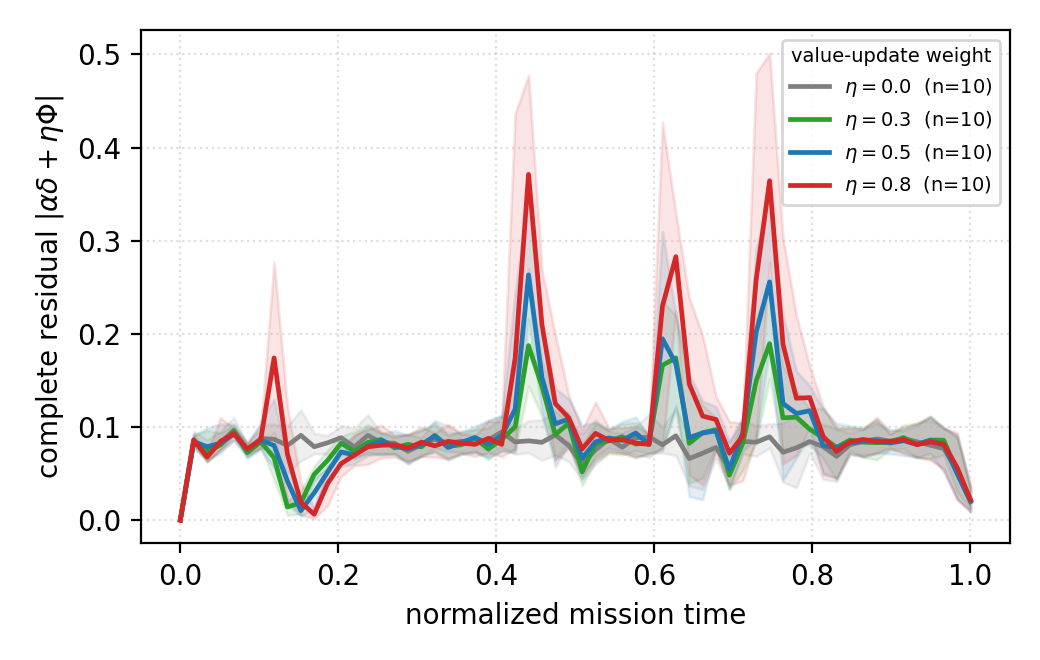
\includegraphics[width=\columnwidth]{qconv}
%% R2#9: "the band is inter-run spread rather than a confidence interval of the
%% mean... it might be worth stating in the caption rather than only in the text,
%% since readers often interpret such bands as inferential."
\caption{Complete update residual $|\alpha\delta+\eta\bm{\Phi}|$ over per-run series
resampled onto a common normalized-time grid, for $\eta\in\{0,0.3,0.5,0.8\}$
(configurations E0, E2, E3, E4). Each curve is the \emph{across-run mean}; the shaded
band is the $2.5$--$97.5$ \emph{percentile band of the per-run series}, that is, the
spread \emph{between runs}---it is \textbf{not} a confidence interval of the mean and
must not be read as one. The residual grows monotonically with $\eta$ while every
discrete behavioral metric is unchanged. For $\eta>0$ the residual is event-driven---flat between
events and spiking during each of the four reactive episodes (one hazard retreat and
three anomaly investigations) as $\eta\bm{\Phi}$ rises and decays, with the band widening
at the peaks---whereas for $\eta=0$ it stays near ${\approx}0.08$ between the
start-up transient and the end-of-mission decline, since the only term left is
$\alpha\delta$. Increments stay bounded (end-of-mission
${\approx}0.020$). The early region ($\lesssim0.2$ normalized time) mixes the
start-up transient with the retreat episode and the across-run alignment there is
loose; we draw no reading from it.}
\label{fig:qconv}
\end{figure}

\paragraph*{The update is affected by $\eta$; the behavior is not}
%% R2#4 pediu que a estabilidade do update fosse atestada no resíduo COMPLETO.
%% A Fig. com sobreposição de eta mostra que o instrumento detecta o termo que
%% deveria detectar -- e que o comportamento não o acompanha. É a afirmação
%% honesta disponível: o update está implementado como especificado e é estável,
%% e nada além disso.
Fig.~\ref{fig:qconv} overlays the complete update residual
$|\alpha\delta+\eta\Phi|$ for $\eta\in\{0,0.3,0.5,0.8\}$. The residual rises
monotonically with $\eta$---peak of the across-run mean $0.097$, $0.189$, $0.263$ and
$0.371$ respectively, with the per-run area under the curve separating completely
between $\eta=0$ and every $\eta>0$ (Cliff's $\delta=1.0$)---while every discrete
behavioral metric is unchanged. This is the expected arithmetic: the residual
contains $\eta\Phi$ by construction, so its growth with $\eta$ is close to
tautological. What the figure establishes is narrower and is all we claim: the update
is implemented as specified and its increments remain bounded and stable over the
mission, and the invariance of behavior is not an artifact of the term being inert in
the table. It says nothing about behavior, which is governed elsewhere.
